% This file was created (at least in part) by the script ParseMdtoLatex by Louis du Plessis
% (Available from https://github.com/taming-the-beast)

\documentclass[11pt]{article}
%%%%%%%%%%%%%%%%%%%%%%%%%%%%%%%%%%%%%%%%%%%%%%%%%%%%%%%%%%%%%%%
% DO NOT EDIT THIS FILE UNLESS YOU KNOW WHAT YOU ARE DOING!!! %
%%%%%%%%%%%%%%%%%%%%%%%%%%%%%%%%%%%%%%%%%%%%%%%%%%%%%%%%%%%%%%%

\usepackage[]{authblk}
\usepackage{graphicx}
\usepackage{color}
\usepackage{longtable}
\usepackage{hanging}
\usepackage{indentfirst}
\usepackage{setspace}
\usepackage{enumitem}
\usepackage{verbatim}
\usepackage{upgreek}
\usepackage{framed}
\usepackage{textcomp}
\usepackage{url}
\usepackage{soul}
\usepackage{amsmath, amsfonts,amssymb,mathrsfs}
\usepackage{fancyhdr}
\usepackage[compact]{titlesec}
\usepackage[T1]{fontenc}
\usepackage{lmodern}

\usepackage[backend=bibtex,hyperref=true,citestyle=authoryear,bibstyle=authortitle,firstinits=true,terseinits=true,doi=false,url=false,eprint=false,maxbibnames=10,maxcitenames=2]{biblatex}
\DeclareCiteCommand{\cite}
  {\usebibmacro{prenote}}
  {\usebibmacro{citeindex}%
   \printtext[bibhyperref]{\usebibmacro{cite}}}
  {\multicitedelim}
  {\usebibmacro{postnote}}

\DeclareCiteCommand*{\cite}
  {\usebibmacro{prenote}}
  {\usebibmacro{citeindex}%
   \printtext[bibhyperref]{\usebibmacro{citeyear}}}
  {\multicitedelim}
  {\usebibmacro{postnote}}

\DeclareCiteCommand{\parencite}[\mkbibparens]
  {\usebibmacro{prenote}}
  {\usebibmacro{citeindex}%
    \printtext[bibhyperref]{\usebibmacro{cite}}}
  {\multicitedelim}
  {\usebibmacro{postnote}}

\DeclareCiteCommand*{\parencite}[\mkbibparens]
  {\usebibmacro{prenote}}
  {\usebibmacro{citeindex}%
    \printtext[bibhyperref]{\usebibmacro{citeyear}}}
  {\multicitedelim}
  {\usebibmacro{postnote}}

\DeclareCiteCommand{\footcite}[\mkbibfootnote]
  {\usebibmacro{prenote}}
  {\usebibmacro{citeindex}%
  \printtext[bibhyperref]{ \usebibmacro{cite}}}
  {\multicitedelim}
  {\usebibmacro{postnote}}

\DeclareCiteCommand{\footcitetext}[\mkbibfootnotetext]
  {\usebibmacro{prenote}}
  {\usebibmacro{citeindex}%
   \printtext[bibhyperref]{\usebibmacro{cite}}}
  {\multicitedelim}
  {\usebibmacro{postnote}}

\DeclareCiteCommand{\textcite}
  {\boolfalse{cbx:parens}}
  {\usebibmacro{citeindex}%
   \printtext[bibhyperref]{\usebibmacro{textcite}}}
  {\ifbool{cbx:parens}
     {\bibcloseparen\global\boolfalse{cbx:parens}}
     {}%
   \multicitedelim}
  {\usebibmacro{textcite:postnote}}

\newcommand{\citep}{\parencite}
\newcommand{\citet}{\textcite}
\defbibheading{relevref}[\refname]{\section*{Relevant References}}

\renewcommand{\postnotedelim}{\iffieldpages{postnote}{\addcolon}{\addcomma\space}} 
\DeclareFieldFormat{postnote}{#1} 

\DeclareFieldFormat[article, inbook, incollection, inproceedings, patent, thesis, unpublished]{title}{#1}
\DeclareFieldFormat[article, inbook, incollection, inproceedings, patent, thesis, unpublished]{journaltitle}{\mkbibemph{#1}\nopunct}
\DeclareFieldFormat[article, inbook, incollection, inproceedings, patent, thesis, unpublished]{volume}{{#1}\addcolon} %puts volume number in parens
%\DeclareFieldFormat[article, inbook, incollection, inproceedings, patent, thesis, unpublished]{year}{\mkbibparens{#1}\nopunct} %puts year in parens

\DeclareFieldFormat[article, incollection, patent, thesis, unpublished]{pages}{{\nopp#1}}

\DeclareFieldFormat{sentencecase}{\MakeSentenceCase{#1}}

\renewbibmacro*{title}{%
  \ifthenelse{\iffieldundef{title}\AND\iffieldundef{subtitle}}
    {}
    {\ifthenelse{\ifentrytype{article}\OR\ifentrytype{inbook}%
      \OR\ifentrytype{incollection}\OR\ifentrytype{inproceedings}%
      \OR\ifentrytype{inreference}}
      {\printtext[title]{%
        \printfield[sentencecase]{title}%
        \setunit{\subtitlepunct}%
        \printfield[sentencecase]{subtitle}}}%
      {\printtext[title]{%
        \printfield[titlecase]{title}%
        \setunit{\subtitlepunct}%
        \printfield[titlecase]{subtitle}}}%
     \newunit}%
  \printfield{titleaddon}}

\DefineBibliographyStrings{english}{% various adjustments to common bib entry strings
urlseen = {Accessed:},% What goes in front of the date a URL was accessed/retrieved etc.
editor = {(Ed)},%Ed – no dot, in brackets
editors = {(Eds)},% Eds – no dot, in brackets
byeditor = {(Ed.)}}% ‘Edited by’ for edited works

\DeclareNameAlias{default}{last-first}

\renewbibmacro{in:}{}

\renewbibmacro{publisher+location+date}{
  \iflistundef{publisher}
    {}
    {\printlist{publisher}%
       {\addcomma\space}%
      \iflistundef{location}
        {}
        {\printlist{location}}%
    }
}

\DeclareBibliographyDriver{article}{%
\usebibmacro{bibindex}%
\usebibmacro{begentry}%
\usebibmacro{author/translator+others}%
\newunit\newblock
\printfield{year}%
\setunit{\labelnamepunct}\newblock
\usebibmacro{title}%
\newunit
\printlist{language}%
\newunit\newblock
\usebibmacro{byauthor}%
\newunit\newblock
\usebibmacro{bytranslator+others}%
\newunit\newblock
\printfield{version}%
\newunit\newblock
%\usebibmacro{in:}% %mit in:
\usebibmacro{journal}%
\newunit\newblock
\printfield{volume}%
\newunit\newblock
\usebibmacro{byeditor+others}%
\newunit\newblock
\usebibmacro{note+pages}%
\newunit\newblock
\iftoggle{bbx:isbn}
{}%
\newunit\newblock
\usebibmacro{doi+eprint+url}%
\newunit\newblock
\usebibmacro{addendum+pubstate}%
\newunit\newblock
\usebibmacro{pageref}%
\usebibmacro{finentry}}

\DeclareBibliographyDriver{inproceedings}{%
\usebibmacro{bibindex}%
\usebibmacro{begentry}%
\usebibmacro{author/translator+others}%
\newunit\newblock
\printfield{year}%
\setunit{\labelnamepunct}\newblock
\usebibmacro{title}%
\newunit
\printlist{language}%
\newunit\newblock
\usebibmacro{byauthor}%
\newunit\newblock
\usebibmacro{bytranslator+others}%
\newunit\newblock
\printfield{version}%
\newunit\newblock
%\usebibmacro{in:}% %mit in:
\usebibmacro{booktitle}%
\newunit\newblock
\printfield{volume}%
\newunit\newblock
\usebibmacro{byeditor+others}%
\newunit\newblock
\usebibmacro{publisher+location+date}%
\newunit\newblock
\usebibmacro{note+pages}%
\newunit\newblock
\usebibmacro{pageref}%
\usebibmacro{finentry}}

\DeclareBibliographyDriver{book}{%
\usebibmacro{bibindex}%
\usebibmacro{begentry}%
\usebibmacro{author/translator+others}%
\newunit\newblock
\printfield{year}%
\setunit{\labelnamepunct}\newblock
\usebibmacro{title}%
\newunit
\printlist{language}%
\newunit\newblock
\usebibmacro{byauthor}%
\newunit\newblock
\usebibmacro{bytranslator+others}%
\newunit\newblock
%\usebibmacro{in:}% %mit in:
\usebibmacro{booktitle}%
\newunit\newblock
\printfield{volume}%
\newunit\newblock
\usebibmacro{publisher+location+date}%
\newunit\newblock
\usebibmacro{note+pages}%
\newunit\newblock
\usebibmacro{pageref}%
\usebibmacro{finentry}}




\setlist{nolistsep}

\setlength{\evensidemargin}{0in}
\setlength{\headheight}{0in}
\setlength{\headsep}{0in}
\setlength{\oddsidemargin}{-0.25in}
\setlength{\paperheight}{11in}
\setlength{\paperwidth}{8.5in}
\setlength{\tabcolsep}{0in}
\setlength{\textheight}{9in}
\setlength{\textwidth}{7in}
\setlength{\topmargin}{0in}
\setlength{\topskip}{0in}
\setlength{\voffset}{0in}
\parskip = 0.15in
\pagestyle{plain}
\setlength{\parindent}{0cm}

\definecolor{citescol}{RGB}{194,101,1}
\definecolor{urlscol}{RGB}{0,150,206}
\definecolor{linkscol}{RGB}{149,0,207}
\definecolor{mycol}{RGB}{25,23,191}
\definecolor{outputcol}{RGB}{34,139,34}
\definecolor{tcol}{RGB}{165,0,14}


\DeclareMathAlphabet{\msfsl}{T1}{cmr}{m}{it}
\DeclareMathAlphabet{\msyf}{OMX}{pcr}{m}{it}
\newcommand{\alf}{\upalpha}
\newcommand{\hilight}[1]{\colorbox{yellow}{#1}}

\newcommand{\levelone}[1]{
\bigskip
\noindent{\LARGE{\textsc{#1}}}
\vspace {0.05in}
}

\newcommand{\leveltwo}[1]{
\bigskip
\noindent{\Large{\textit{#1}}}
\vspace {-1mm}
}

\newcommand{\descriptionhead}[1]{
\noindent{\textcolor{mycol}{\textbf{\textit{#1}}}}\\ \vspace{-7mm}
}

\newcommand{\dhead}[1]{
\noindent{\textbf{\textit{#1 --}}}
}



\newcommand{\exs}[1]{
\vspace{-4mm}
\begin{itemize}
\item #1 \\ \vspace{-8mm}
\end{itemize}
}

\newcommand{\nbo}[1]{{\color{red}{#1}}}


\newcommand{\stepbullet}{\noindent \textbullet \ }
\newcommand{\mi}[1]{\textbf{\textit{#1}}}


\newcommand{\levelthree}[1]{\textit{#1 --}}


%\bibliographystyle{apalike}
%\bibpunct[; ]{(}{)}{;}{a}{,}{;}


\usepackage[breaklinks]{hyperref}
\usepackage[all]{hypcap}
\hypersetup{colorlinks=true,linkcolor=linkscol,citecolor=citescol,urlcolor=urlscol}


\newcommand{\R}{\texttt{R} }
\newcommand{\TESS}{\texttt{TESS}}
\newcommand{\PBD}{\texttt{PBD}}
\newcommand{\DDD}{\texttt{DDD}}
\newcommand{\Laser}{\texttt{laser}}
\newcommand{\TreePar}{\texttt{TreePar}}
\newcommand{\diversitree}{\texttt{diversitree}}
\newcommand{\RevBayes}{\texttt{RevBayes}}
\newcommand{\Rev}{\texttt{Rev}}
\newcommand{\MrBayes}{\texttt{MrBayes}}
\newcommand{\BEAST}{\texttt{BEAST}}
\newcommand{\PhyloBayes}{\texttt{PhyloBayes}}
\newcommand{\PAML}{\texttt{PAML}}

\let\otheriint\iint
\let\iint\relax
\usepackage{ wasysym }

\usepackage{framed}
\usepackage[]{listings}
%\usepackage{fontspec}
\usepackage{placeins}
\usepackage{epstopdf}



\lstset{backgroundcolor=\color[rgb]{0.972,0.972,0.972},
		tabsize=4,
		rulecolor=,
        basicstyle=\scriptsize,
        upquote=true,
        aboveskip={1.5\baselineskip},
        columns=fixed,
        showstringspaces=false,
        extendedchars=true,
        breaklines=true,
        prebreak = \raisebox{0ex}[0ex][0ex]{\ensuremath{\hookleftarrow}},
        frame=single,
        showtabs=false,
        showspaces=false,
        showstringspaces=false,
        identifierstyle=\ttfamily,
        keywordstyle=\color[rgb]{0,0,1},
        commentstyle=\color[rgb]{0.133,0.545,0.133},
        stringstyle=\color[rgb]{0.627,0.126,0.941}
}

\definecolor{shadecolor}{RGB}{194,225,255}

\setlength{\tabcolsep}{5pt}
\setlength{\topmargin}{-0.4in}
\setlength{\headheight}{14.5pt}
\pagestyle{fancy}

\newcommand{\taha}[1]{{\textcolor{red}{[TAH comment: #1]}}} % TAH comment

\titlespacing{\section}{0pt}{*0}{*0}
\titlespacing{\subsection}{0pt}{*0}{*0}
\titlespacing{\subsubsection}{0pt}{*0}{*0}

\titleformat{\section}
  {\normalfont\Large\bfseries\color{mycol}}
  {\thesection}{1em}{}

\titleformat{\subsection}
  {\normalfont\large\bfseries\color{mycol}}
  {\thesubsection}{1em}{}

\titleformat{\subsubsection}
  {\normalfont\bfseries\color{mycol}}
  {\thesubsubsection}{1em}{}

% command for MrBayes command-line step
\newcommand{\cl}[1]{{\texttt{\textbf{#1}}}}

\newcommand{\colx}[1]{{\textcolor{tcol}{#1}}}

\newcommand{\mbcl}[1]{\exs{\cl{MrBayes > {#1}}}}

\newcommand{\rbprmt}{RevBayes > } 
\newcommand{\rbcl}[1]{\exs{\cl{\rbprmt{#1}}}}
\newcommand{\rbout}[1]{\exs{\cl{\textcolor{outputcol}{#1}}}}
\newcommand{\rbdn}{{\Large \symbol{126}}} % This makes a copy/pasteable tilde
\newcommand{\rbclml}[1]{\exs{\cl{\ \ \ \ \ \ \ \ \ \ \ {#1}}}}

% text box settings
% requires compiling w/ XeLaTeX
%\newfontfamily\listingsfont[Scale=1.0]{Courier New}
%\lstset{basicstyle=\listingsfont, columns=texcl}
%\defaultfontfeatures{Mapping=tex-text}


\makeatletter
\lst@CCPutMacro\lst@ProcessOther {"2D}{\lst@ttfamily{-{}}{-{}}}
\@empty\z@\@empty
\makeatother


\usepackage{tikz}

\setlength{\topmargin}{-0.4in}
\setlength{\headheight}{14.5pt}
\pagestyle{fancy}

\usepackage[breaklinks]{hyperref}
\usepackage[all]{hypcap}
\hypersetup{colorlinks=true,linkcolor=linkscol,citecolor=citescol,urlcolor=urlscol}

\definecolor{lg}{gray}{0.75}
\def\gcirc{{%
    \setbox0\hbox{$\fullmoon$}%
    \rlap{\hbox to \wd0{\hss{$\textcolor{lg}{\newmoon}$}\hss}}\box0
}}



% Add your bibtex library here
\addbibresource{master-refs}


%%%%%%%%%%%%%%%%%%%%
% Do NOT edit this %
%%%%%%%%%%%%%%%%%%%%
\begin{document}
\renewcommand{\headrulewidth}{0.5pt}
\headsep = 20pt
\lhead{ }
\rhead{\textsc {BEAST v2 Tutorial}}
\thispagestyle{plain}


%%%%%%%%%%%%%%%%%%
% Tutorial title %
%%%%%%%%%%%%%%%%%%
\begin{center}

	% Enter the name of your tutorial here
	\textbf{\LARGE Tutorial using BEAST v2.7.x}\\\vspace{2mm}

	% Enter a short description of your tutorial here
	\textbf{\textcolor{mycol}{\Large Troubleshooting}}\\

	\vspace{4mm}

	% Enter the names of all the authors here
	{\Large {\em David A. Rasmussen}}
\end{center}



%%%%%%%%%%%%%%%%%
% Tutorial body %
%%%%%%%%%%%%%%%%%

\hypertarget{background}{%
\section{Background}\label{background}}

The primary goal of most phylogenetic analyses in BEAST is to infer the
posterior distribution of trees and associated model parameters using
Markov chain Monte Carlo (MCMC) sampling. In this tutorial, we will
learn how to analyze the output of an MCMC analysis in BEAST2 using
Tracer. This program allows us to easily visualize BEAST's output and
summarize results. As we will see, we can also use Tracer to
troubleshoot some of the most common MCMC problems encountered in BEAST.

While BEAST's MCMC algorithm is fairly well optimised for phylogenetic
inference, problems can arise, especially as the complexity of our data
and models increase. An MCMC run may not converge on a stationary target
distribution. More commonly, a run might converge but mix poorly -
meaning that our samples from the posterior are highly autocorrelated
and therefore not independent. In these cases, it is often necessary to
tune the performance of the MCMC algorithm.

In this tutorial, we will consider a relatively simple example where we
would like to infer a phylogeny and evolutionary parameters from a small
alignment of sequences. Our job will be to work together to increase the
efficiency of the MCMC so we can make BEAST purr\ldots{} \clearpage

\hypertarget{programs-used-in-this-exercise}{%
\section{Programs used in this
Exercise}\label{programs-used-in-this-exercise}}

\hypertarget{beast2---bayesian-evolutionary-analysis-sampling-trees-2}{%
\subsubsection{BEAST2 - Bayesian Evolutionary Analysis Sampling Trees
2}\label{beast2---bayesian-evolutionary-analysis-sampling-trees-2}}

BEAST2 (\url{http://www.beast2.org}) is a free software package for
Bayesian evolutionary analysis of molecular sequences using MCMC and
strictly oriented toward inference using rooted, time-measured
phylogenetic trees. This tutorial is written for BEAST v2.7.x \citep{Bouckaert2014, Bouckaert2019}.

\hypertarget{beauti2---bayesian-evolutionary-analysis-utility}{%
\subsubsection{BEAUti2 - Bayesian Evolutionary Analysis
Utility}\label{beauti2---bayesian-evolutionary-analysis-utility}}

BEAUti2 is a graphical user interface tool for generating BEAST2 XML
configuration files.

Both BEAST2 and BEAUti2 are Java programs, which means that the exact
same code runs on all platforms. For us it simply means that the
interface will be the same on all platforms. The screenshots used in
this tutorial are taken on a Mac OS X computer; however, both programs
will have the same layout and functionality on both Windows and Linux.
BEAUti2 is provided as a part of the BEAST2 package so you do not need
to install it separately.

\hypertarget{tracer}{%
\subsubsection{Tracer}\label{tracer}}

Tracer (\url{http://beast.community/tracer}) is used to summarise the
posterior estimates of the various parameters sampled by the Markov
Chain. This program can be used for visual inspection and to assess
convergence. It helps to quickly view median estimates and 95\% highest
posterior density intervals of the parameters, and calculates the
effective sample sizes (ESS) of parameters. It can also be used to
investigate potential parameter correlations. We will be using Tracer
v1.7.x.

\clearpage

\hypertarget{practical-getting-beast-to-purr}{%
\section{Practical: Getting BEAST to
purr}\label{practical-getting-beast-to-purr}}

\hypertarget{the-data}{%
\subsection{The data}\label{the-data}}

To get started, I have generated a XML file that we can run our
phylogenetic analysis in BEAST.

\begin{framed}
Download the first \textbf{BEAST2} input file
\passthrough{\lstinline!tutorial\_run1.xml!}
\end{framed}

The XML contains an alignment of 36 randomly simulated DNA sequences.

\hypertarget{inspecting-the-xml-file-in-beauti}{%
\subsection{Inspecting the XML file in
BEAUti}\label{inspecting-the-xml-file-in-beauti}}

While we can open the XML file in any standard text editor, BEAUTi
offers an easy way to inspect the different elements of the analysis:

\begin{framed}
Open \textbf{BEAUti} and load in the
\passthrough{\lstinline!tutorial\_run1.xml!} file by navigating to
\textbf{File \textgreater{} Load}.
\end{framed}

By navigating between the different tabs at the top of the application
window, we can inspect the data and each element of the analysis. For
example, in the \textbf{Site Model} panel, we can see that we are
fitting a GTR substitution model with no gamma rate heterogeneity
(Figure \ref{fig:beauti_run1}).

\begin{figure}
    \centering
    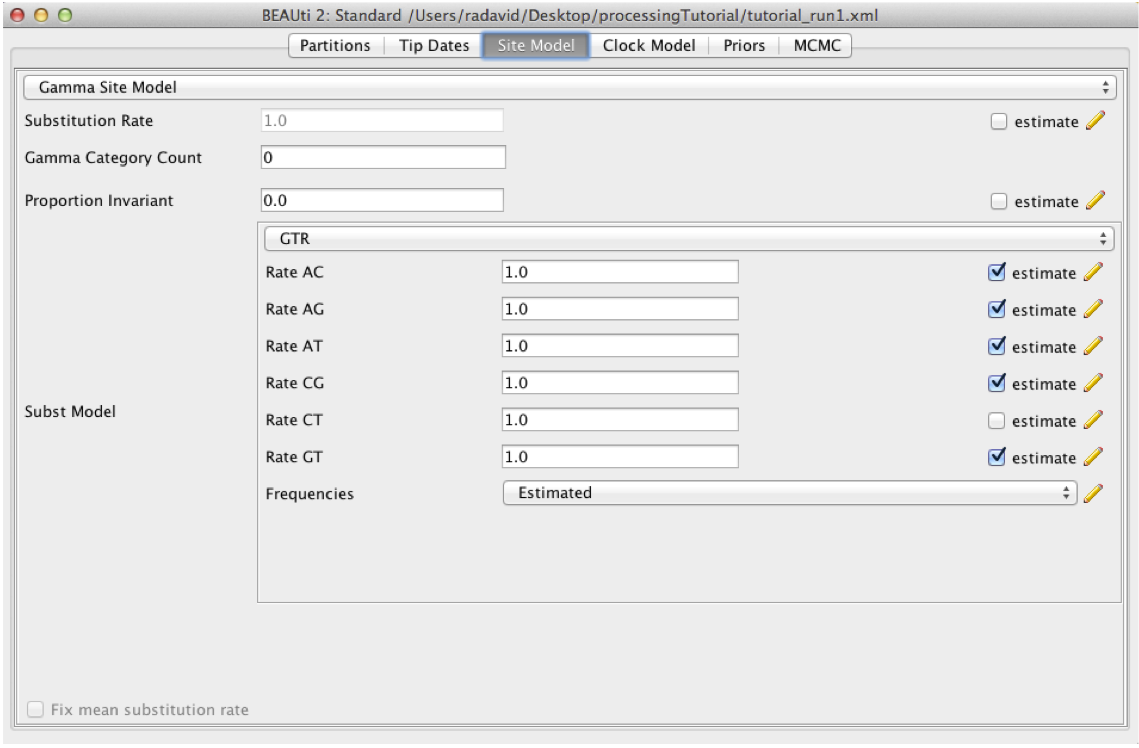
\includegraphics[width=0.800000\textwidth]{figures/beauti_run1.png}
    \caption{The Site Model panel in BEAUTi}
    \label{fig:beauti_run1}
\end{figure}

\hypertarget{running-the-xml-in-beast}{%
\subsubsection{Running the XML in
BEAST}\label{running-the-xml-in-beast}}

We are now ready to run our first analysis in BEAST.

\begin{framed}
Open \textbf{BEAST2} and choose
\passthrough{\lstinline!tutorial\_run1.xml!} as the Input file. Then
click \textbf{Run}.
\end{framed}

\begin{figure}
    \centering
    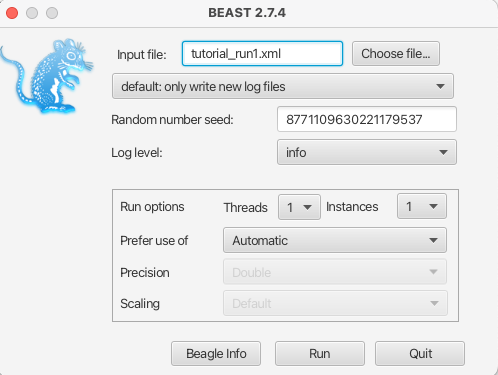
\includegraphics[width=0.500000\textwidth]{figures/beast_input_run1.png}
    \caption{Running BEAST with the specified XML configuration file.}
    \label{fig:beast_run1}
\end{figure}

Since we are only running 200,000 iterations, the MCMC should finish
running in under 30 seconds.

\hypertarget{visualizing-beasts-output-in-tracer}{%
\subsubsection{Visualizing BEAST's output in
Tracer}\label{visualizing-beasts-output-in-tracer}}

\begin{framed}
Open \textbf{Tracer} and navigate to \textbf{File \textgreater{} Import
Trace File}, then open \passthrough{\lstinline!tutorial\_run1.log!}
\textbf{or} simply drag and drop the file into the \textbf{Tracer}
window.
\end{framed}

The results of your run will look similar, but not necessarily
identical, to my results shown in Figure \ref{fig:beast_run1}.

Tracer allows us to quickly visualize BEAST's MCMC output in order to
check performance and see our parameter estimates. On the left there is
a panel where all model parameters are listed along with their mean
posterior estimates and Effective Sample Size (ESS). Recall that the ESS
tells us how many pseudo-independent samples we have from the posterior,
so the higher the better. Here, we can see that the ESS is low for all
parameters, indicating that we do not yet have a good estimate of the
posterior distribution.

By selecting a parameter in the left panel and then clicking on the
\textbf{Trace} tab, we can see how the MCMC explored parameter space
(Figure \ref{fig:tracer_run1}). For the \textbf{clockRate} parameter for
instance, we see that the chain quickly converged to a value of about
0.01 (the true value used to simulate the sequence data), but mixing was
poor, hence the low ESS.

\begin{figure}
    \centering
    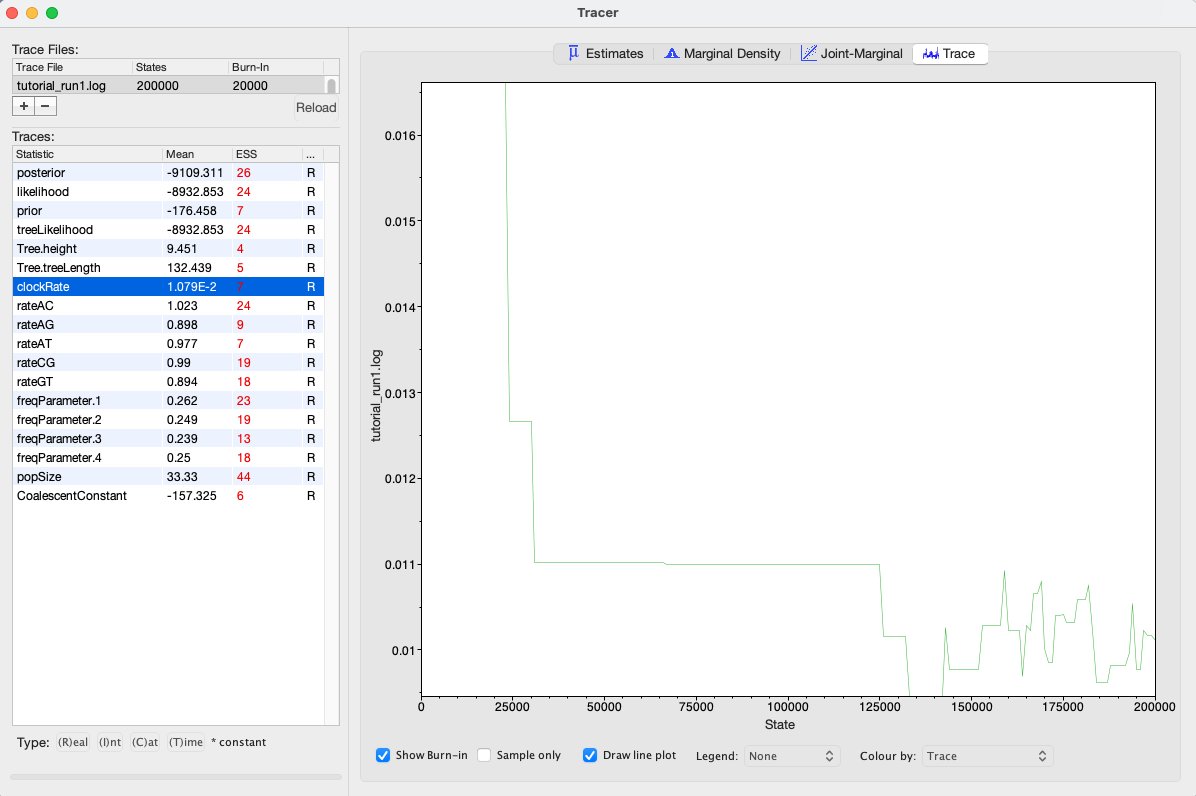
\includegraphics[width=0.800000\textwidth]{figures/tracer_run1.png}
    \caption{A trace plot for the clockRate parameter}
    \label{fig:tracer_run1}
\end{figure}

We can also see our posterior estimates for each parameter by clicking
on the \textbf{Estimates} tab while highlighting the desired parameter
in the left panel. This provides us with various summary statistics and
a frequency histogram representing our estimate of the posterior
distribution constructed from our MCMC samples. For the
\textbf{clockRate} parameter, we can see that our estimate of the
posterior is extremely rough, again because we have so few uncorrelated
samples from the posterior (Figure \ref{fig:tracer_run1_ests}).

\begin{figure}
    \centering
    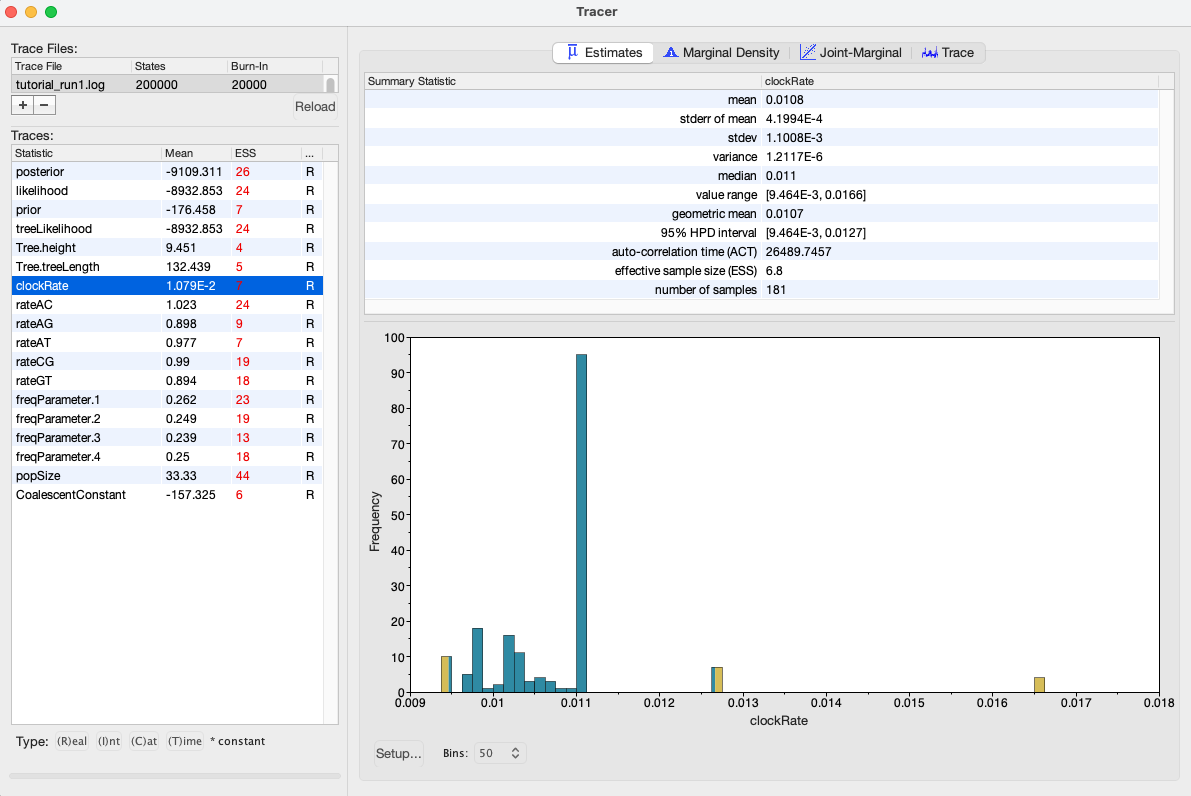
\includegraphics[width=0.800000\textwidth]{figures/tracer_run1_ests.png}
    \caption{Posterior estimates of the clockRate in Tracer.}
    \label{fig:tracer_run1_ests}
\end{figure}

\hypertarget{run-2-increasing-the-chain-length}{%
\subsubsection{Run 2: Increasing the chain
length}\label{run-2-increasing-the-chain-length}}

By checking the ESS, trace plots and parameter estimates, we got the
picture that none of our parameters in Run 1 mixed well. In this case,
the simplest thing to try is to rerun the MCMC for more iterations.

\begin{framed}
Load \passthrough{\lstinline!tutorial\_run1.xml!} back into
\textbf{BEAUti} using \textbf{File \textgreater{} Load}. Navigate to the
MCMC panel and increase the chain length to 1 million. When done,
navigate \textbf{File \textgreater{} Save As} and save as
\passthrough{\lstinline!tutorial\_run2.xml!}.
\end{framed}

Note that we didn't need to change the file names fo the
\textbf{tracelog} or \textbf{treelog}, since they are by default set to
\passthrough{\lstinline!$(filebase).log!} and
\passthrough{\lstinline!$(filebase)-$(tree).trees!}. When running the
analysis \passthrough{\lstinline!$(filebase)!} will be replaced by the
name of the XML file and \passthrough{\lstinline!$(tree)!} by the name
of tree in the analysis (in this case the name of the alignment).

\begin{framed}
Run the \passthrough{\lstinline!tutorial\_run2.xml!} file in
\textbf{BEAST2} as we did before. When done, open
\passthrough{\lstinline!tutorial\_run2.log!} in \textbf{Tracer}.
\end{framed}

Looking at the MCMC output in Tracer, we see that increasing the chain
length did help (Figure \ref{fig:tracer_run2}). The ESS values are
higher and the traces look better, but still not great. In the next
section, we will continue to focus on the \textbf{clockRate} parameter
because it still has a low ESS and appears to mix especially poorly.

\begin{figure}
    \centering
    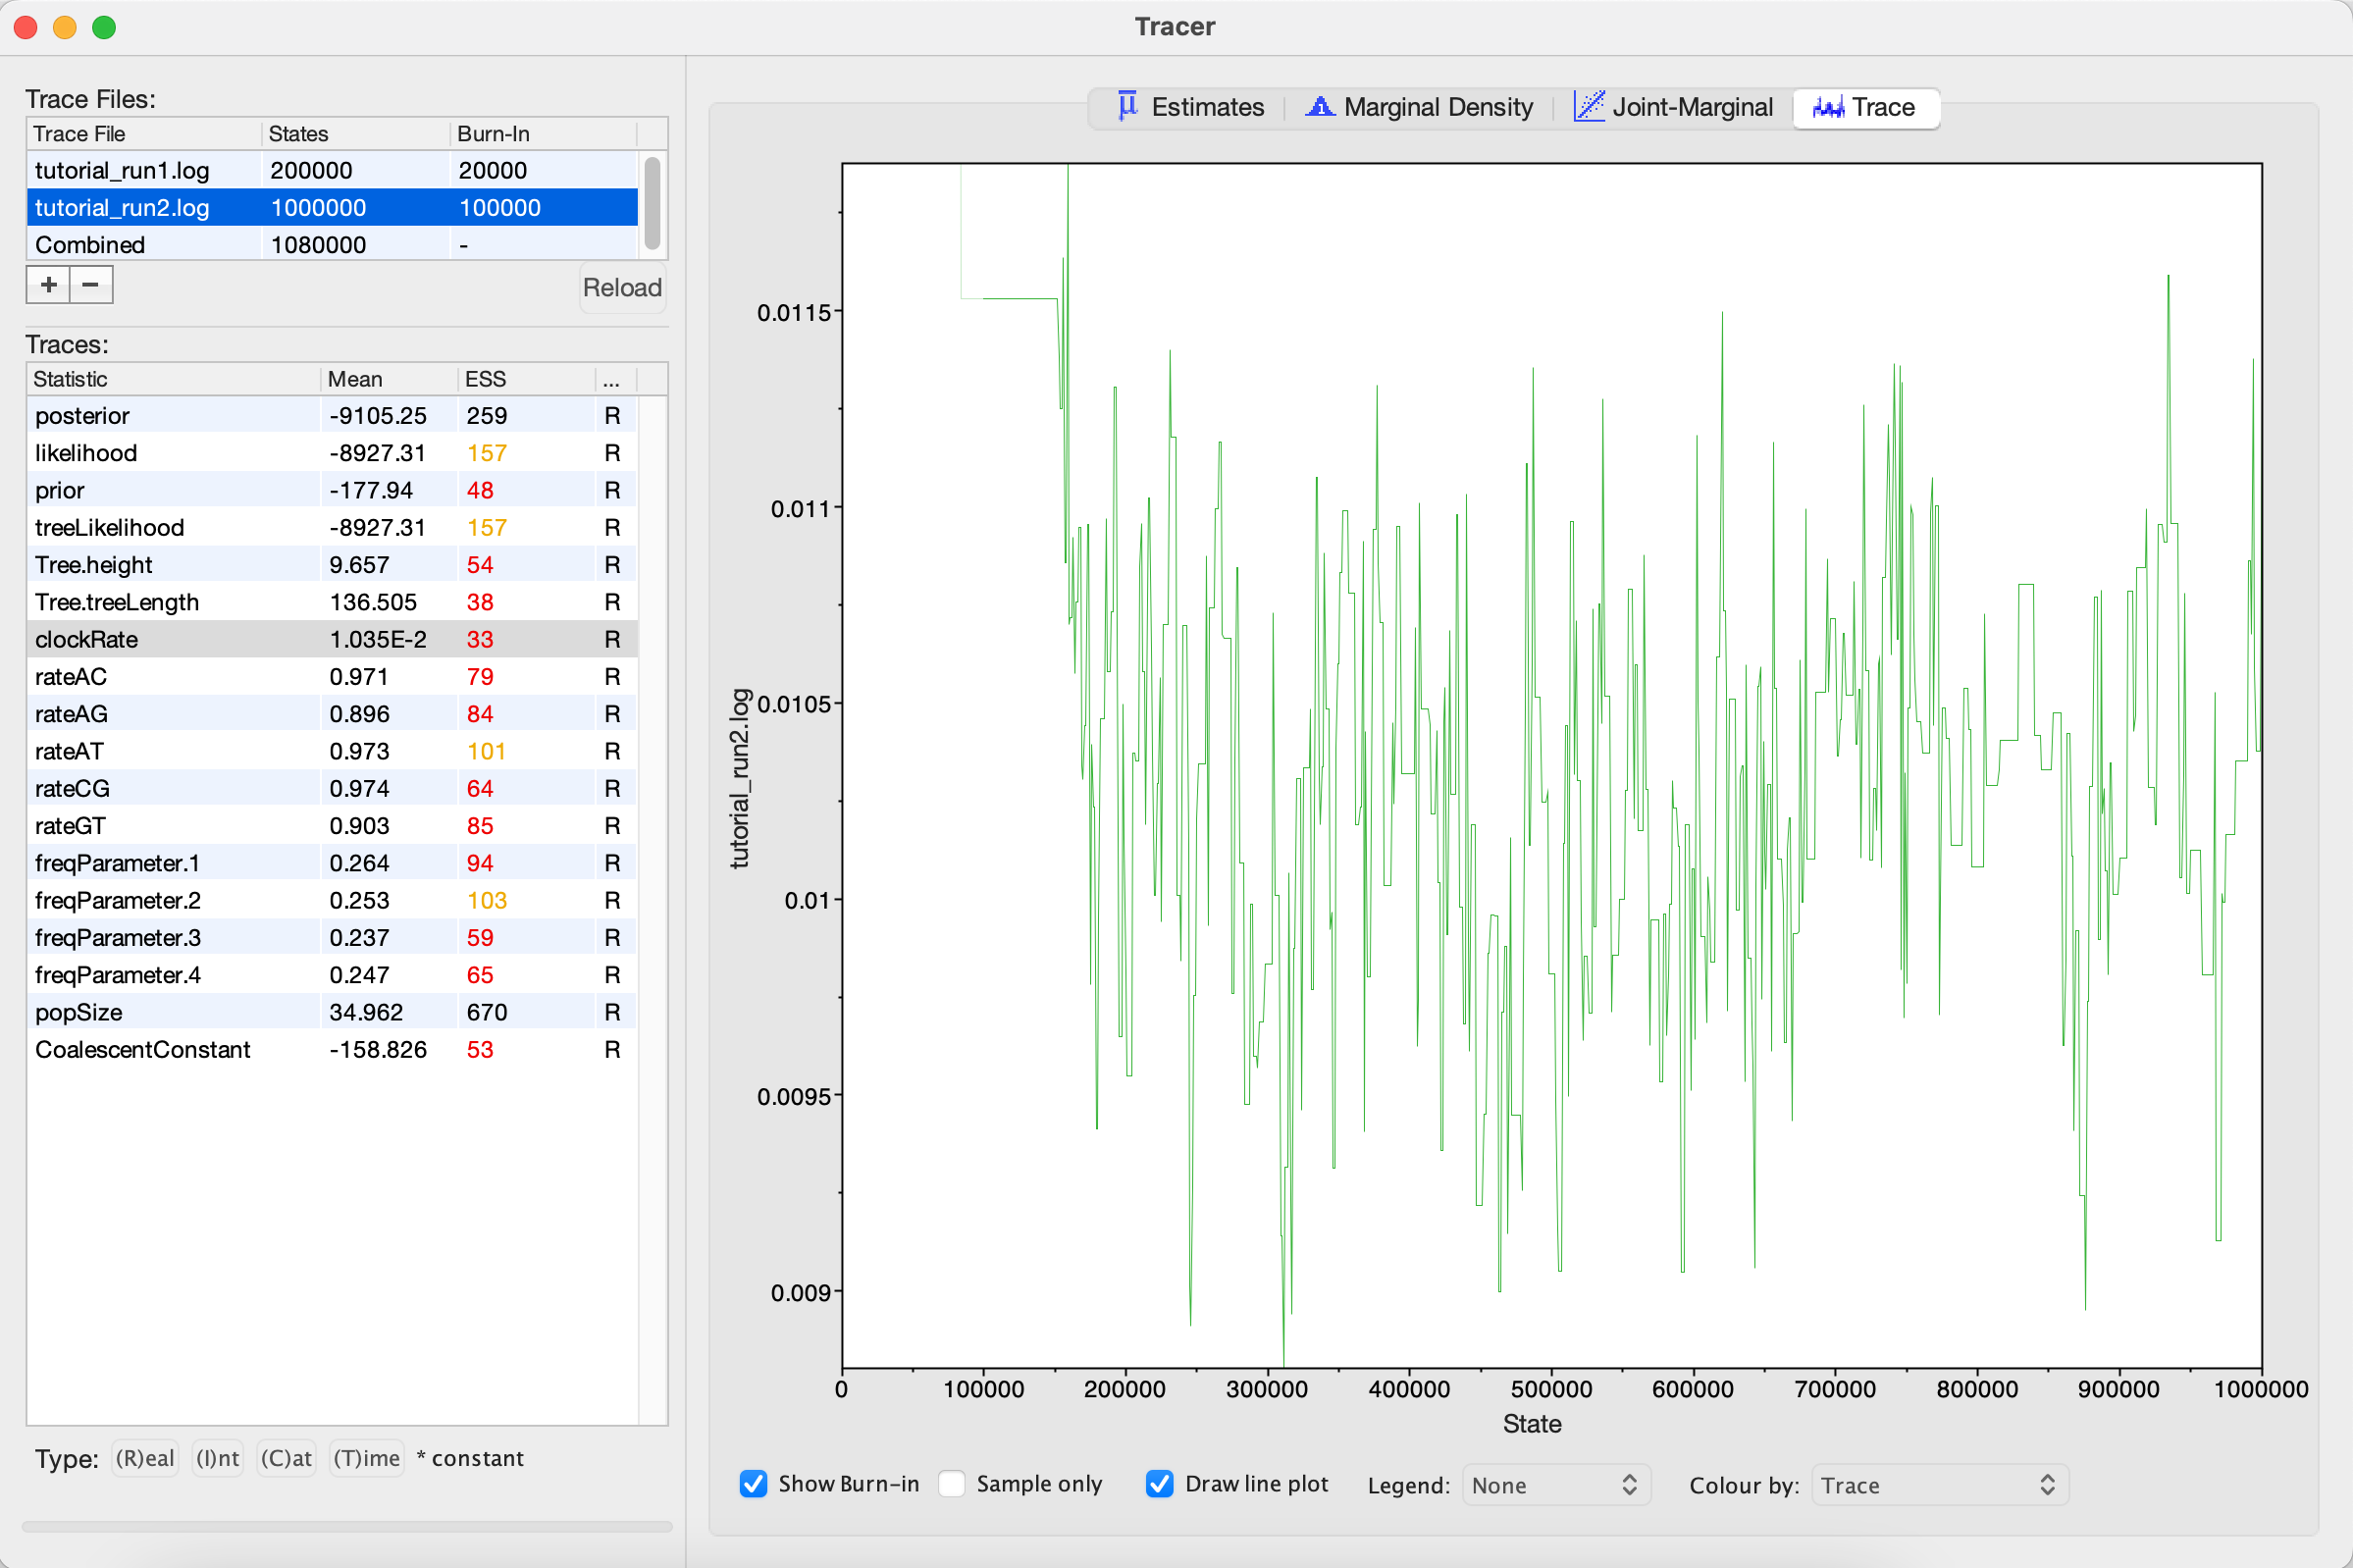
\includegraphics[width=0.800000\textwidth]{figures/tracer_run2.png}
    \caption{A trace plot for the clockRate parameter}
    \label{fig:tracer_run2}
\end{figure}

\hypertarget{run-3-changing-the-clockrate-operators}{%
\subsubsection{\texorpdfstring{Run 3: Changing the \textbf{clockRate}
operators}{Run 3: Changing the clockRate operators}}\label{run-3-changing-the-clockrate-operators}}

If one parameter in particular is not converging or mixing well, we can
try to tweak that parameter's operator(s). Remember that BEAST's
operators control what new parameter values are proposed at each MCMC
iteration and how these proposals are made (i.e.~the proposal
distribution). Since the \textbf{clockRate} parameter was not mixing
well in Run 2, we will try increasing the frequency at which new
\textbf{clockRates} are proposed.

\begin{framed}
Load \passthrough{\lstinline!tutorial\_run2.xml!} back into
\textbf{BEAUti} and select \textbf{View \textgreater{} Show Operators
panel}. This will bring up a new panel showing all the operators in use
(Figure \ref{fig:beauti_run3}). In the box to the right of
\passthrough{\lstinline!Adaptable Sampler: clockRate.c:seqs  Scale substitution rate of partition c:seqs!},
change the value from \textbf{0.05} to \textbf{3.0}. When done, save as
\passthrough{\lstinline!tutorial\_run3.xml!}.
\end{framed}

\begin{figure}
    \centering
    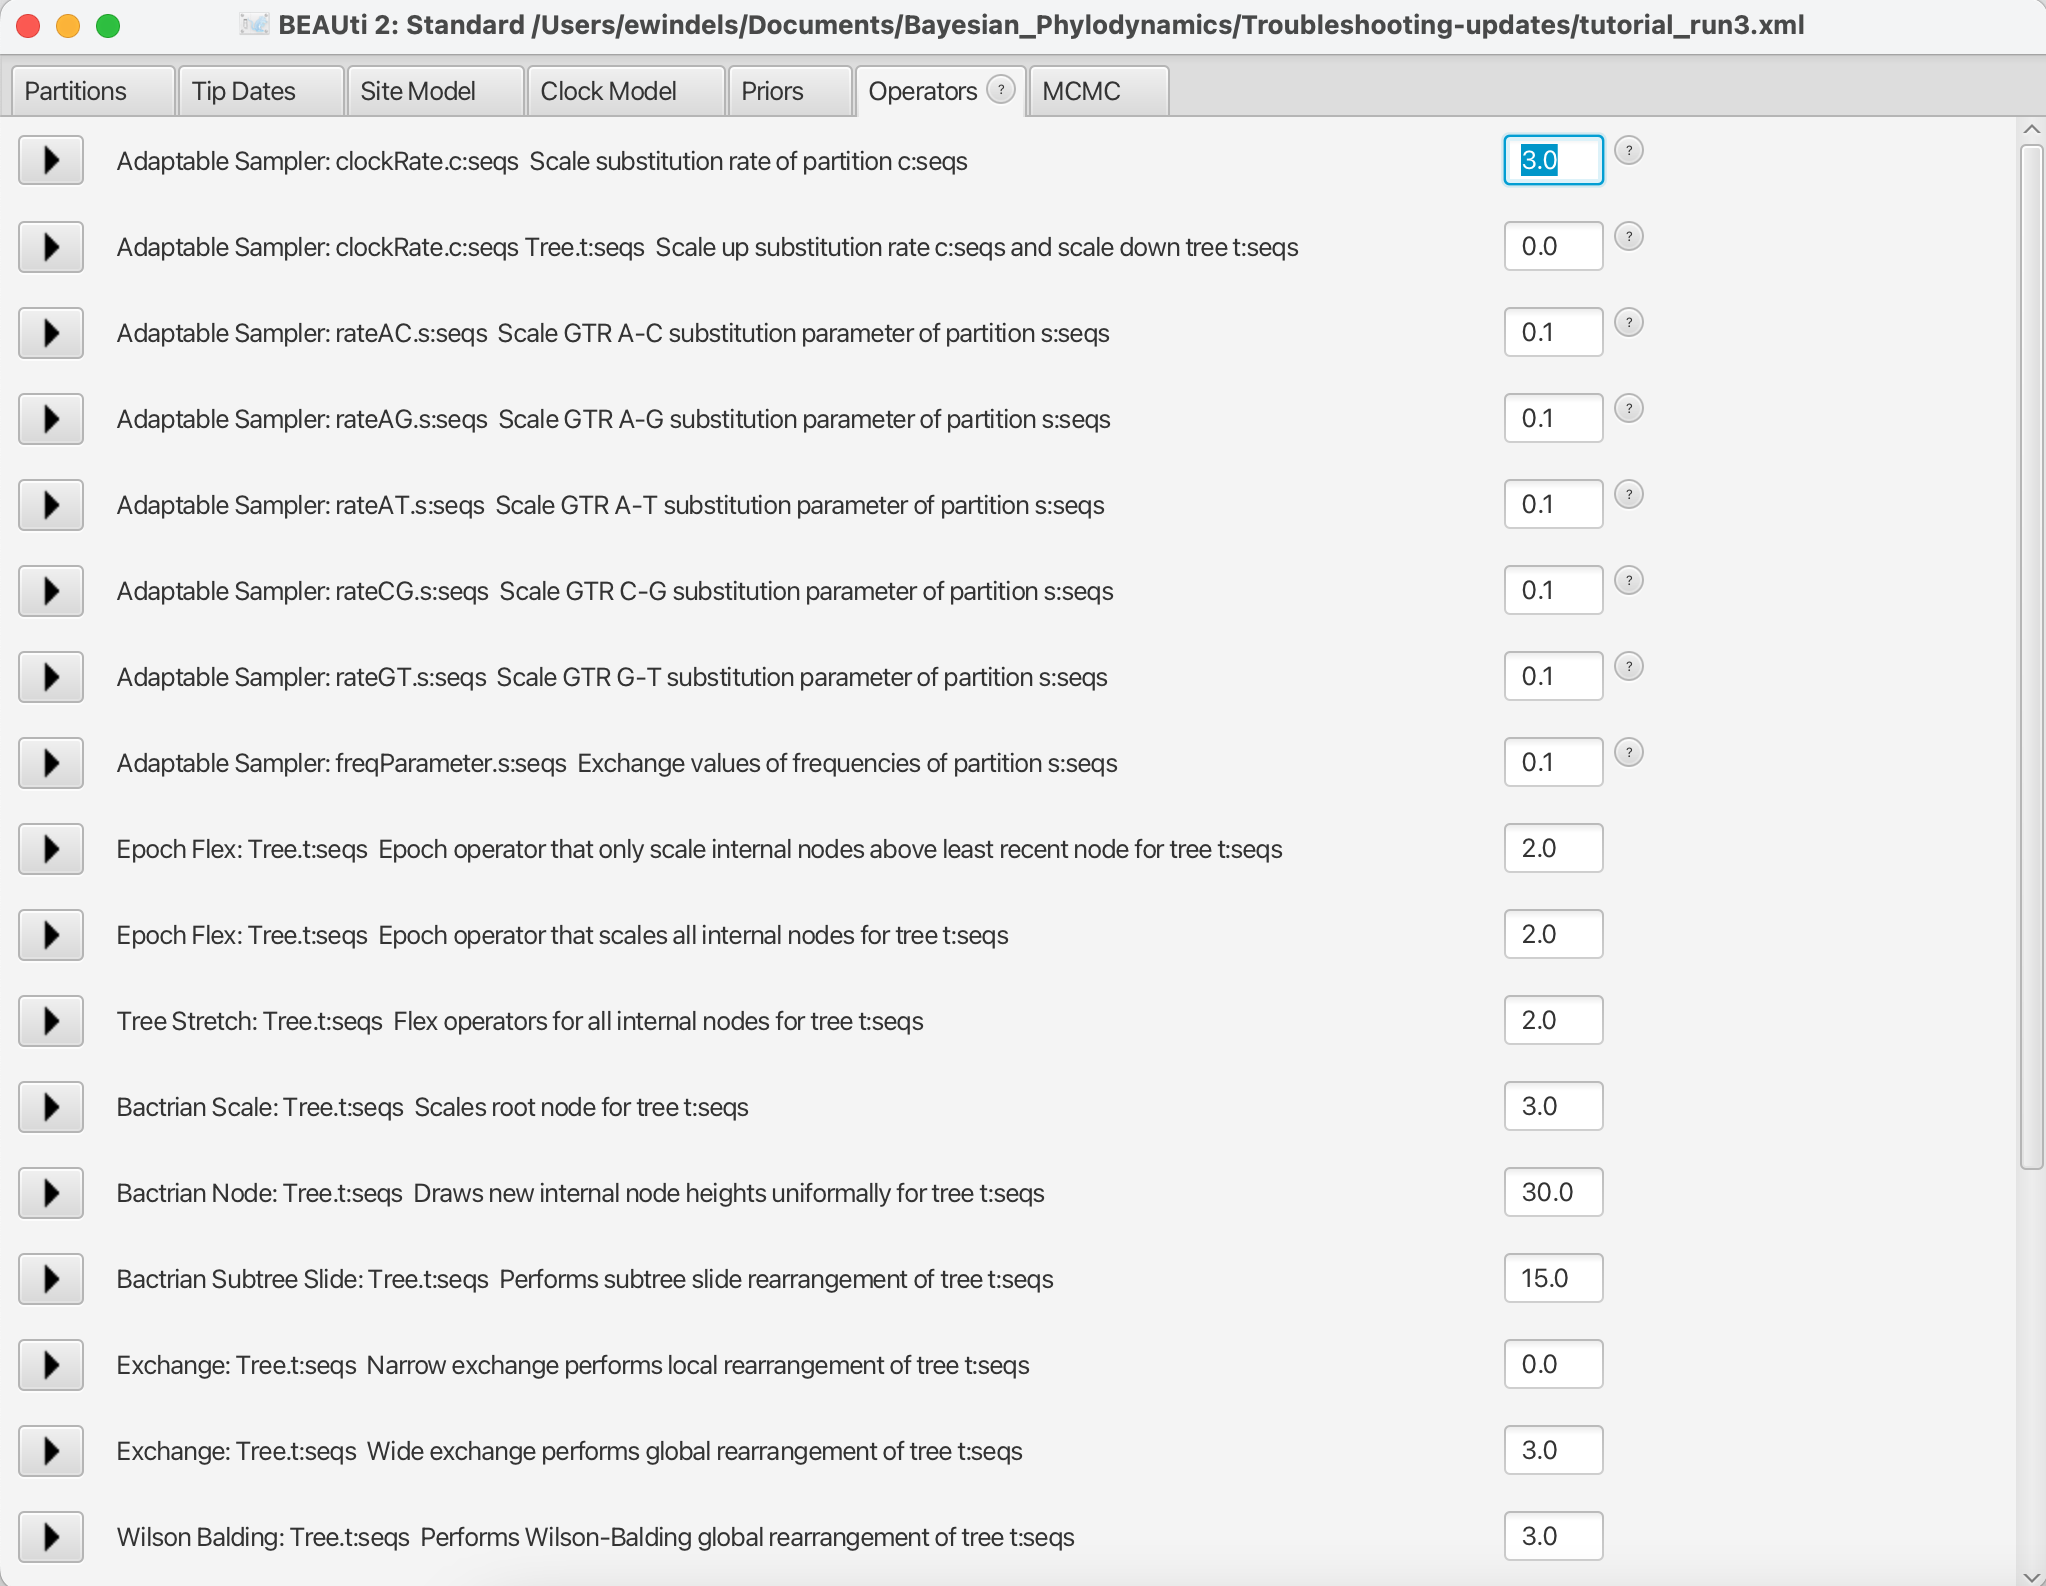
\includegraphics[width=0.800000\textwidth]{figures/beauti_run3.png}
    \caption{The Operators panel in BEAUTi}
    \label{fig:beauti_run3}
\end{figure}

So, what just happened? We increased the weight of the scale operator on
the \textbf{clockRate}, which moves the parameter value up or down, so
that new \textbf{clockRates} will be proposed more often in the MCMC.
Going from a weight of 0.05 to 3.0 means that new proposals for that
parameter will be made sixty times as often, but the frequency at which
a given operator is called depends on the weights given to other
operators. So if there are parameters with very high ESS values, we may
want to reallocate weight on their operators to operators on less well
mixing parameters.

\begin{framed}
Run \passthrough{\lstinline!tutorial\_run3.xml!} in \textbf{BEAST2} and
then open \passthrough{\lstinline!tutorial\_run3.log!} in
\textbf{Tracer}.
\end{framed}

We can see that optimizing the operator dramatically improves mixing for
the \textbf{clockRate} (Figure \ref{fig:tracer_run3}).

\begin{figure}
    \centering
    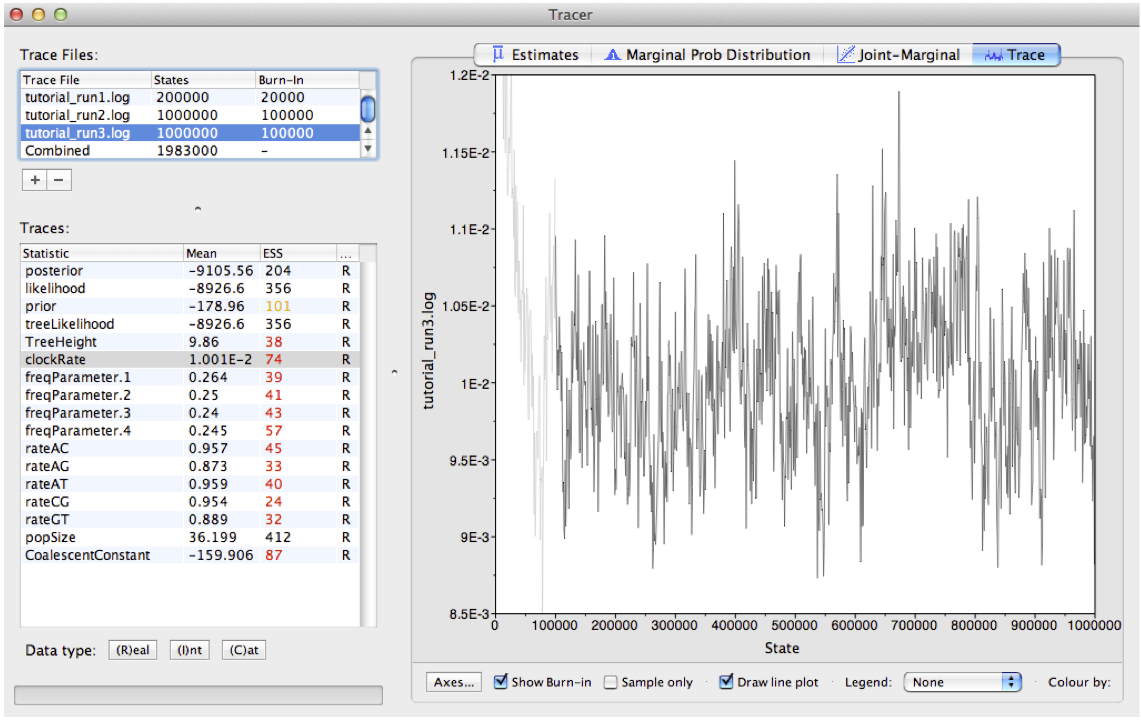
\includegraphics[width=0.800000\textwidth]{figures/tracer_run3.png}
    \caption{A trace plot for the clockRate parameter}
    \label{fig:tracer_run3}
\end{figure}

One thing to keep in mind is that BEAST is using MCMC to explore a
multidimensional parameter space, and poor mixing in one dimension can
be caused by poor mixing in another dimension. This often arises because
two parameters are highly correlated. We can identify these correlations
in Tracer by visualizing the joint distribution of a pair of parameters
together. To do this, select one parameter in the left panel and then,
while holding the command key (Mac) or control key (Windows), select
another. Then click on the \textbf{Joint-Marginal} tab at the top and
uncheck the \textbf{Sample only} box at the bottom. Looking at the
pairwise joint distribution for \textbf{Tree.height} and
\textbf{clockRate}, we see that these two parameters are highly
negatively correlated (Figure \ref{fig:tracer_run3Joint}). We therefore
may want to add an operator that updates these parameters together to
more efficiently explore their parameter space.

\begin{figure}
    \centering
    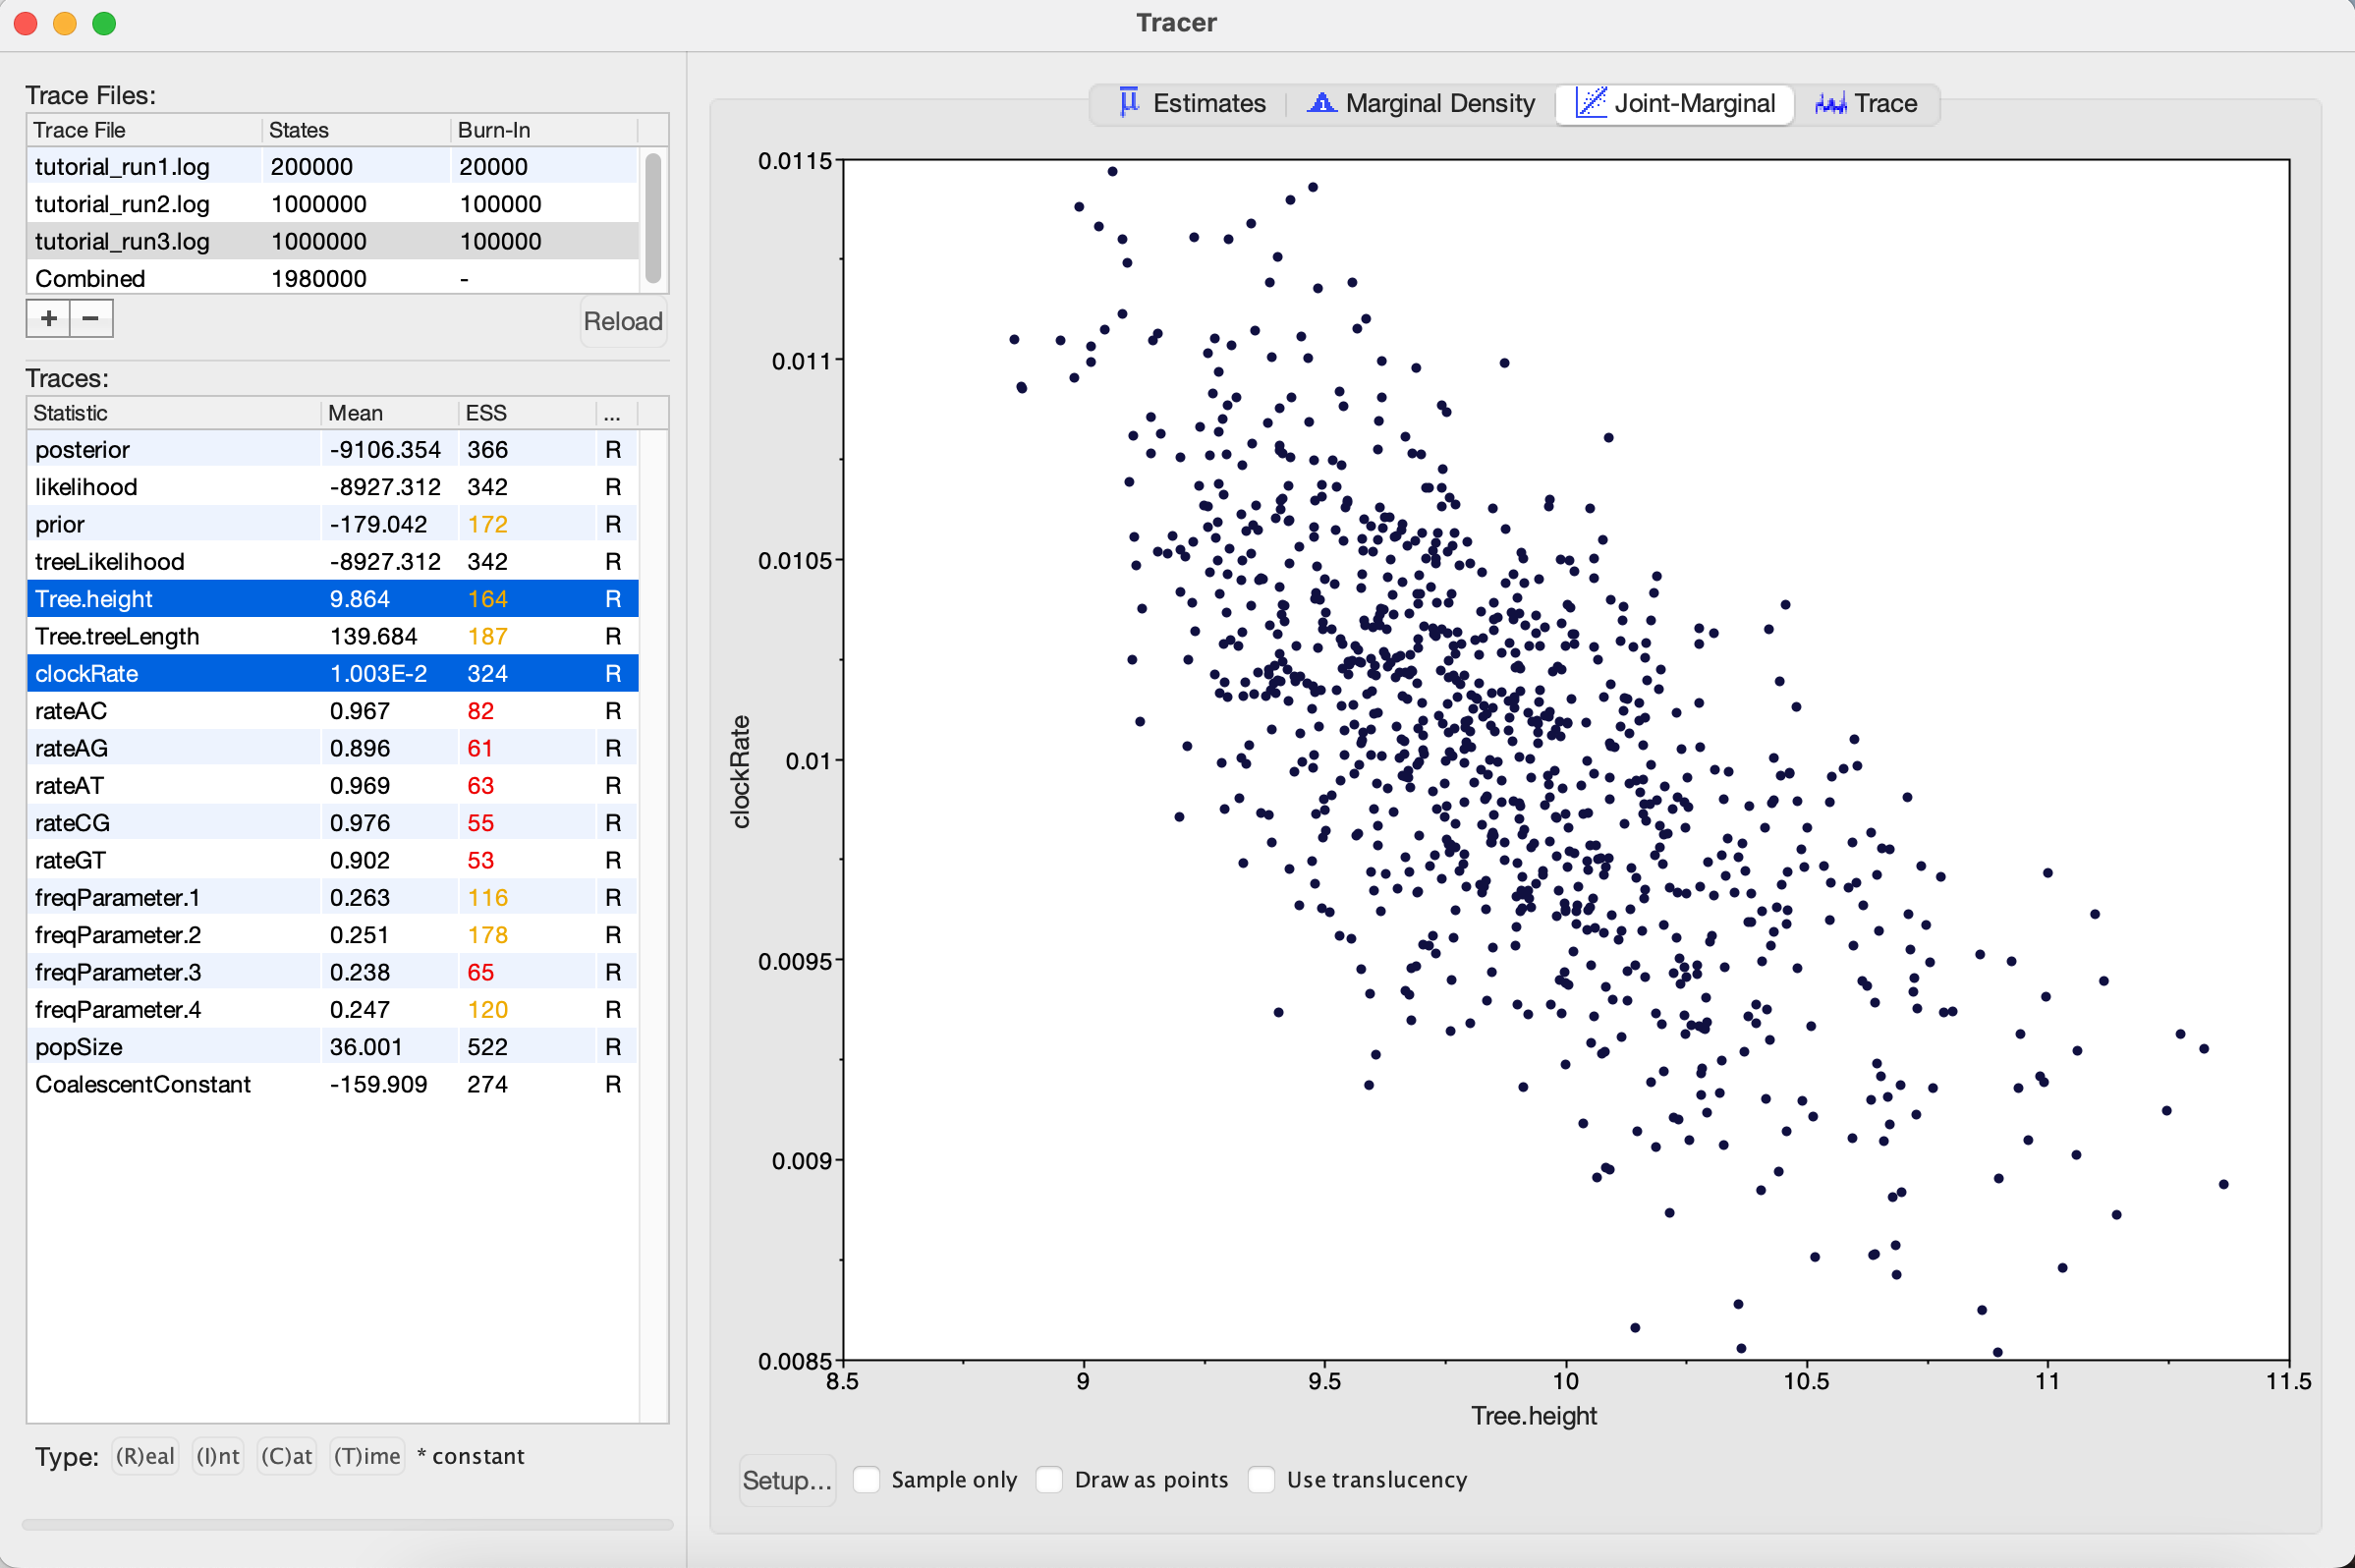
\includegraphics[width=0.800000\textwidth]{figures/tracer_run3Joint.png}
    \caption{The joint posterior distribution of Tree.height and clockRate}
    \label{fig:tracer_run3Joint}
\end{figure}

\hypertarget{run-4-adding-an-updown-operator}{%
\subsubsection{Run 4: Adding an UpDown
operator}\label{run-4-adding-an-updown-operator}}

The easiest way to improve MCMC performance when two parameters are
highly negatively correlated is to add an \textbf{UpDown} operator. This
operator scales one parameter up while scaling the other parameter down.
If two parameters are highly positively correlated we can also use this
operator to scale both parameters in the same direction, up or down.

\begin{framed}
Load \passthrough{\lstinline!tutorial\_run3.xml!} back into
\textbf{BEAUti} and select \textbf{View \textgreater{} Show Operators
panel} as before. In the box to the right of
\passthrough{\lstinline!Adaptable Sampler: clockRate.c:seqs Tree.t:seqs  Scale up substitution rate c:seqs and scale down tree t:seqs!},
change the weight on the \textbf{Bactrian UpDown} operator from
\textbf{0.0} to \textbf{3.0}. When done, save as
\passthrough{\lstinline!tutorial\_run4.xml!}.
\end{framed}

We just added an \textbf{UpDown} operator on the \textbf{clockRate} and
the \textbf{Tree.height} parameters. The fact that these two parameters
are highly negatively correlated makes perfect sense. An increase in the
\textbf{clockRate} means that less time is needed for substitutions to
accumulate along branches; meaning branches can be shorter and yet still
explain the same amount of accumulated evolutionary change in the
sequence data. If all branches in the tree become shorter, then the
total \textbf{Tree.height} will also decrease. Thus, it makes sense to
include an \textbf{UpDown} operator on \textbf{clockRate} and
\textbf{Tree.height}. In fact, by default BEAUTi includes this operator.
However, I disabled it in the original XML file by setting the weight on
this operator to zero for the purpose of illustration.

\begin{framed}
Run \passthrough{\lstinline!tutorial\_run4.xml!} in \textbf{BEAST2} and
then open \passthrough{\lstinline!tutorial\_run4.log!} in
\textbf{Tracer}.
\end{framed}

Looking at the MCMC output in Tracer, we see that all parameters are
starting to mix well with relatively high ESS values. Personally, I
would probably want to run one final MCMC for several million iterations
just to be on the safe side, but this can easily be done by adding more
iterations to the chain as we did for Run 2. Alternatively, multiple
different MCMC runs can be combined using the program LogCombiner that
comes packaged with BEAST. This may be better than running one single
long analysis, as it allows us to be sure independent runs are
converging on posterior parameter values and increases our confidence
that we are sampling from the equilibrium distribution.

\begin{figure}
    \centering
    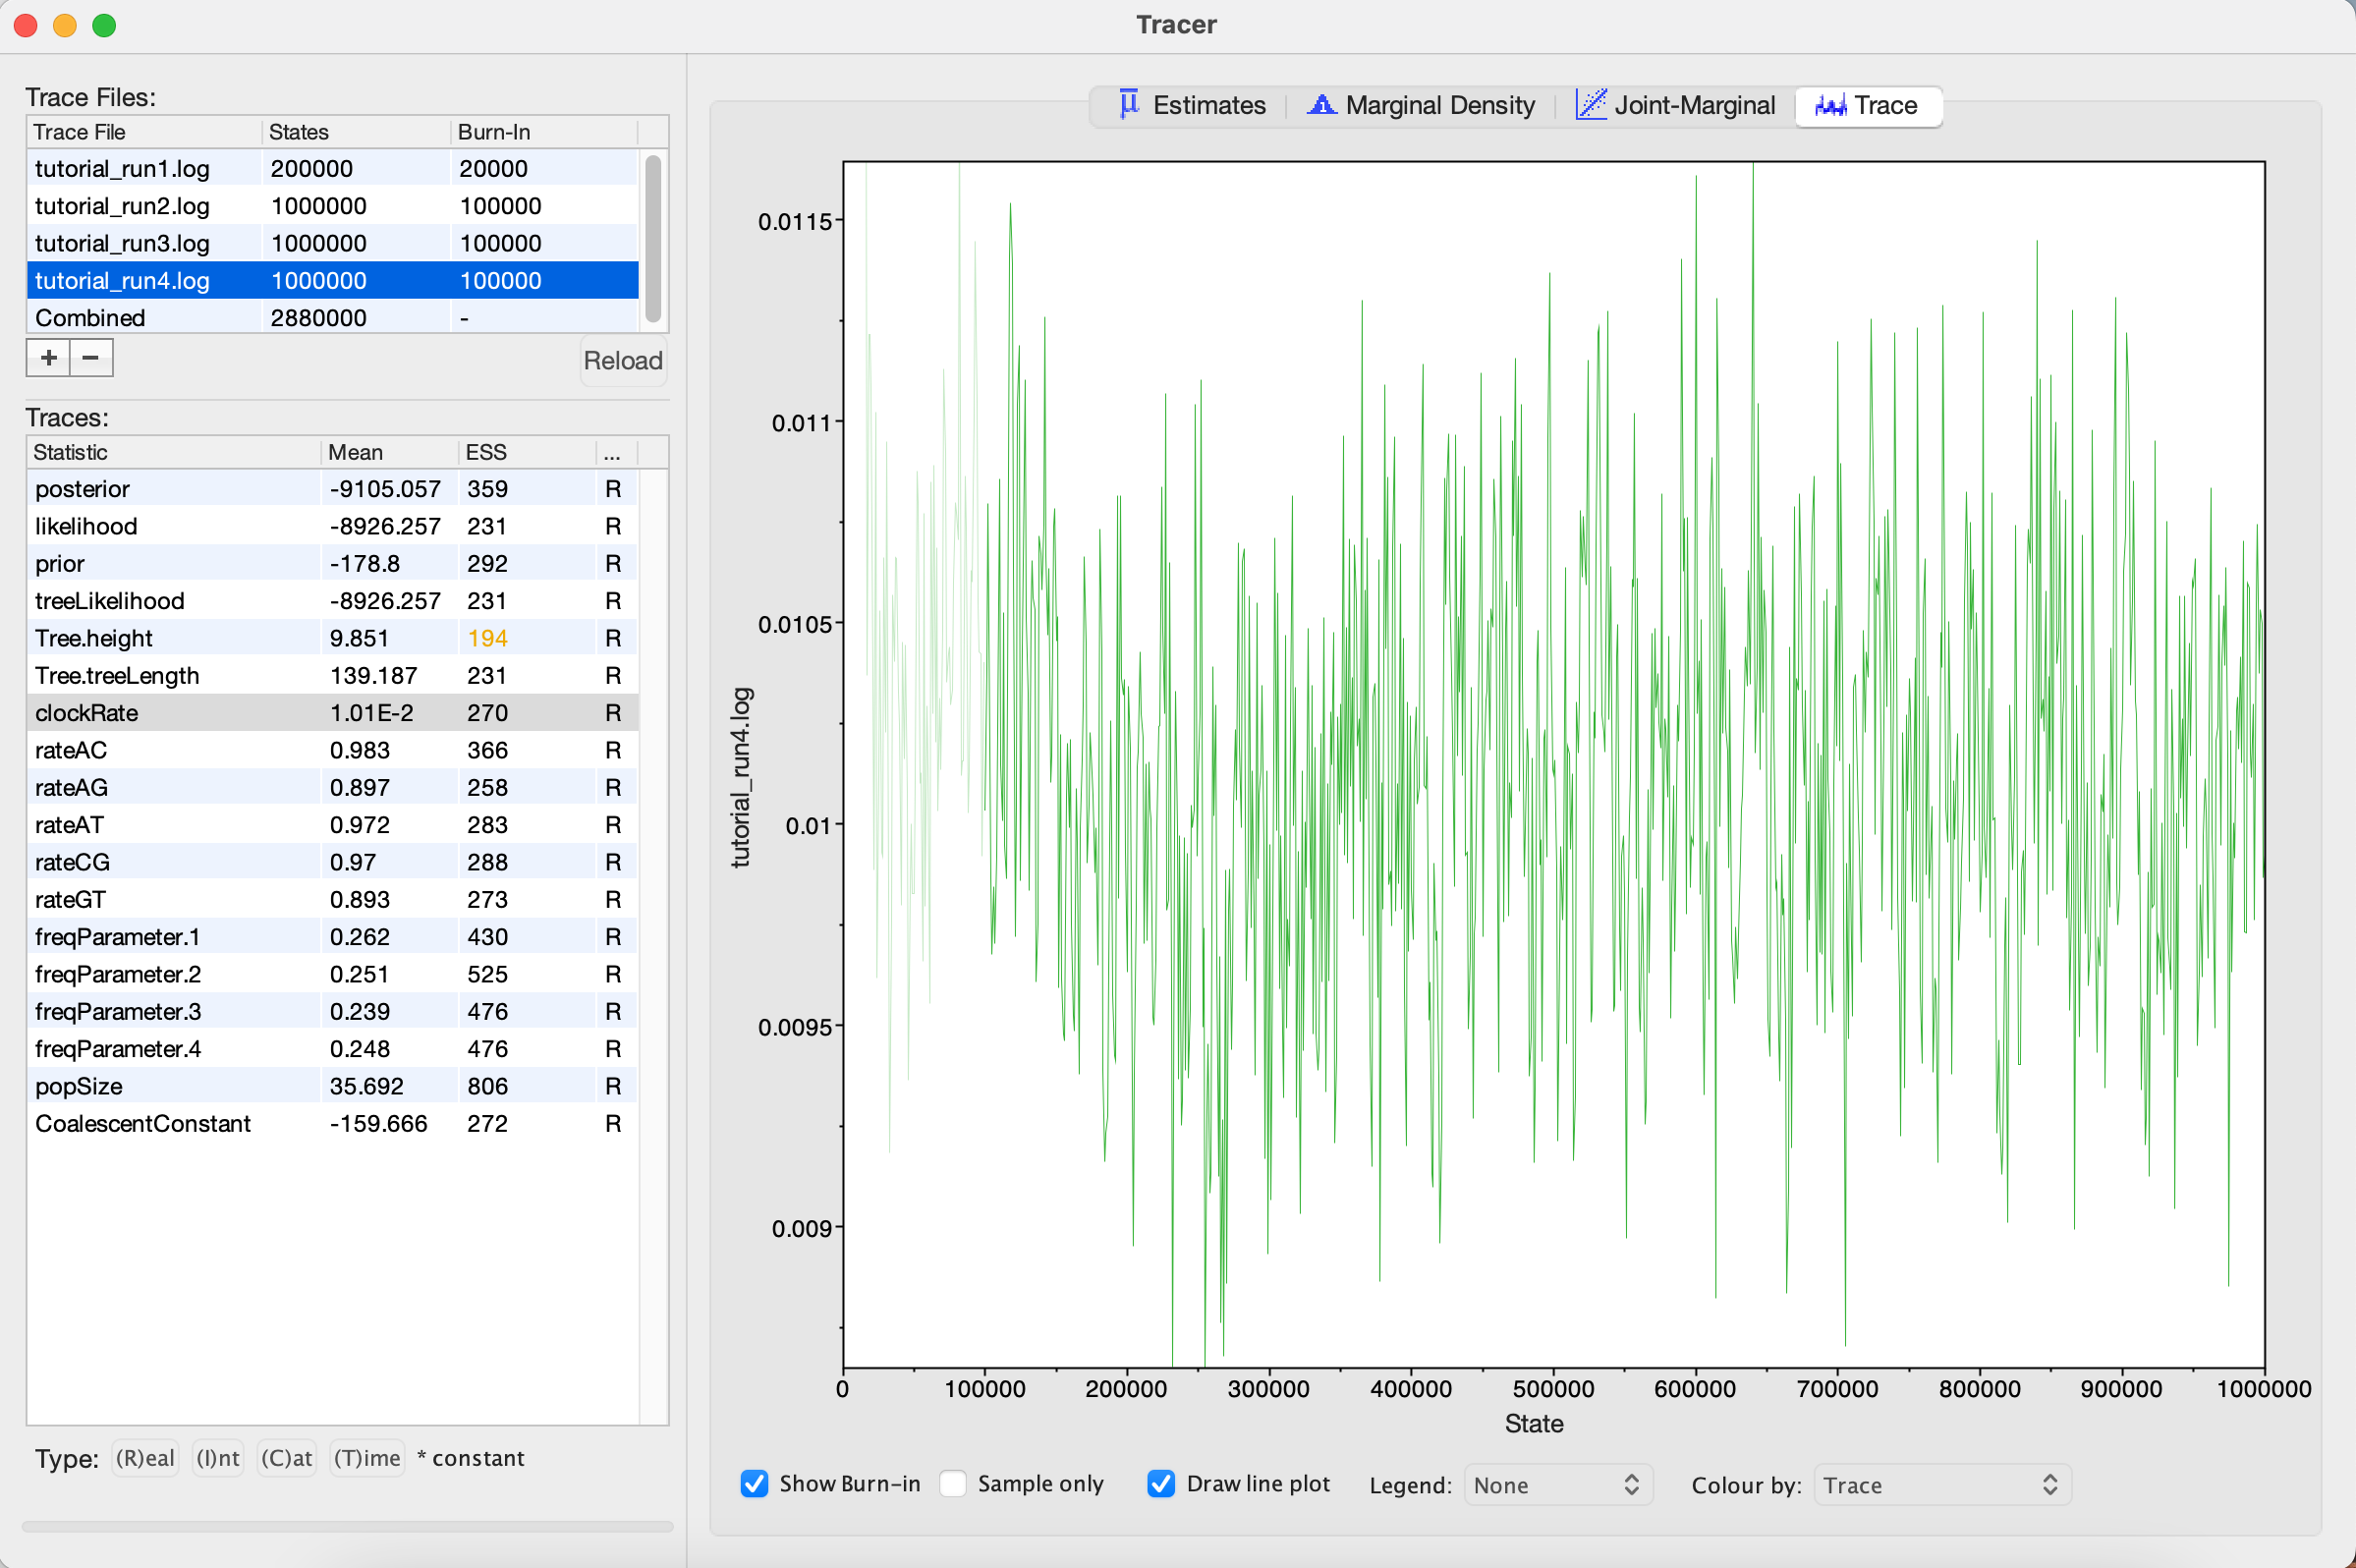
\includegraphics[width=0.800000\textwidth]{figures/tracer_run4.png}
    \caption{A trace plot for the clockRate parameter}
    \label{fig:tracer_run4}
\end{figure}

\hypertarget{further-things-to-keep-in-mind}{%
\subsubsection{Further things to keep in
mind}\label{further-things-to-keep-in-mind}}

\begin{itemize}

\item
  The number of MCMC iterations needed to achieve a reasonable posterior
  sample in this tutorial was quite small. With larger alignments, much
  longer chains may be needed.
\item
  In this tutorial we only considered MCMC performance with respect to
  exploring parameter space, but we also need to consider tree space.
  One simple diagnostic for checking convergence and mixing in tree
  space is to look at the trace plot for the tree likelihood. Poor
  mixing in the tree likelihood can indicate problems exploring tree
  space.
\item
  It is always a good idea to check your posterior estimates against
  sampling from the prior.
\end{itemize}

\hypertarget{useful-links}{%
\section{Useful Links}\label{useful-links}}

\begin{itemize}

\item
  \href{http://www.beast2.org/book.html}{\emph{Bayesian Evolutionary
  Analysis with BEAST 2; chapter 10.}} \citep{BEAST2book2014}
\end{itemize}

\clearpage

\hypertarget{relevant-references}{%
}

%%%%%%%%%%%%%%%%%%%%%%%
% Tutorial disclaimer %
%%%%%%%%%%%%%%%%%%%%%%%
% Please do not change the license
% Add the author names and relevant links
% Add any other aknowledgments here
\href{http://creativecommons.org/licenses/by/4.0/}{
\includegraphics[scale=0.8]{figures/ccby.pdf}} This tutorial was written by David
A.
Rasmussen for \href{https://taming-the-beast.github.io}{Taming the BEAST} and is licensed under a \href{http://creativecommons.org/licenses/by/4.0/}{Creative Commons Attribution 4.0 International License}. 


%%%%%%%%%%%%%%%%%%%%
% Do NOT edit this %
%%%%%%%%%%%%%%%%%%%%
Version dated: \today



\newpage

%%%%%%%%%%%%%%%%
%  REFERENCES  %
%%%%%%%%%%%%%%%%

\printbibliography[heading=relevref]


\end{document}